\subsection{SRGAN}

El SISR (Single Image Super Resolution) es un problema inverso, \emph{it est}, que para una imagen de baja resolución puede haber muchas
imágenes diferentes de alta resolución que le correspondan, esto basado en la interpretación del método utilizado, ya que
el principio básico es añadir información para obtener imágenes de alta resolución.
Las CNN presentan un gran avance en la reconstrucción de imágenes de baja resolución a alta resolución,
sin embargo, debido al escalado de la imagen o el hecho de que la imagen que se busca mejorar presenta grandes
variaciones con respecto a las del dataset (\emph{Data Augmentation}) los resultados podrían ser no satisfactorios.


Una alternativa que propone un nuevo paradigma son las GAN´s (Generative Adversarial Networks), cuyo funcionamiento está basado
en la estimación de modelos generadores, como mencionan Goodfellow et al. \cite{GANs}, esto es 
posible gracias al entrenamiento simultáneo de dos modelos, uno \emph{generador (G)} que obtiene 
la distribución de la entrada para generar datos falsos y el otro \emph{discriminador (D)} el cual se encarga de estimar 
la probabilidad de que la muestra provenga del dataset de entrenamiento y discernir así entre estos datos y 
los del modelo \emph{ generador (G)}.

El término \emph{antagónicas} como se menciona en \cite{SRGAN_Tesis}, se refiere a la dinámica 
competitiva que se mantiene entre los dos modelos. Por un lado,
el generador tiene por objetivo crear nuevos datos que sean indistinguibles del
conjunto de entrenamiento, mientras que el discriminador debe poder ser capaz
de distinguir cuáles son los datos creados y los reales, siendo los últimos los que corresponden
 al conjunto de entrenamiento. Esto resulta en un proceso iterativo donde estos dos modelos
 se desafían uno a otro, logrando un ajuste de parámetros
 que logran producir datos que se parezcan con gran acierto a los reales.
 

\begin{figure}[H]
    \begin{center}
      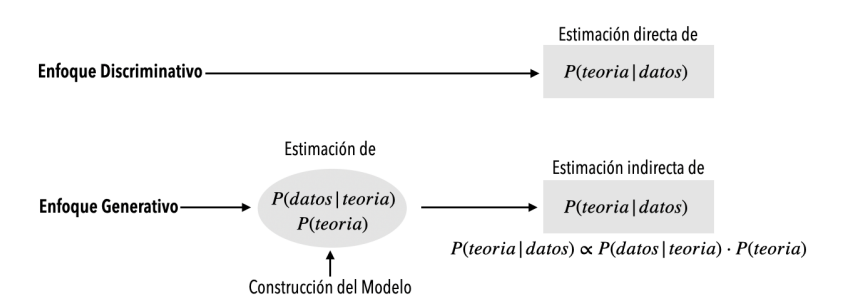
\includegraphics[scale = 0.9]{modelo_gen_disc.png}
      \caption{Modelo Generador y Discriminador}
      \label{Alexis1}
    \end{center}
\end{figure}

\subsubsection{Componentes.}

Profundizando un poco más en los componentes del algoritmo, en especifico, el uso de las \emph{GAN´s} para la obtención de Super-Resolución (\emph{SRGAN}), 
tenemos al discriminador el cual es una red neuronal convolucional que consta de muchas 
capas ocultas y una capa de salida, la principal diferencia aquí es que la capa de salida de las GAN puede tener solo dos salidas, 
a diferencia de las CNN, que pueden tener un número diferente de salidas con respecto a la cantidad de etiquetas en las que está entrenado.
La salida del discriminador puede ser 1 o 0 dependiendo de la función de activación que se aplique. Si la salida es 1, 
entonces los datos proporcionados son reales y si la salida es 0, entonces se refiere a ellos como datos falsos.

El discriminador está capacitado con los datos del dataset, con estos aprende a reconocer cómo se ven y qué características deben 
clasificarse como reales, formalmente, discrimina entre $\tilde{x}$, la muestra falsa, y $x$, 
los datos muestreados de la distribución real de datos $P_{datos}(x)$.




\begin{figure}[H]
    \begin{center}
      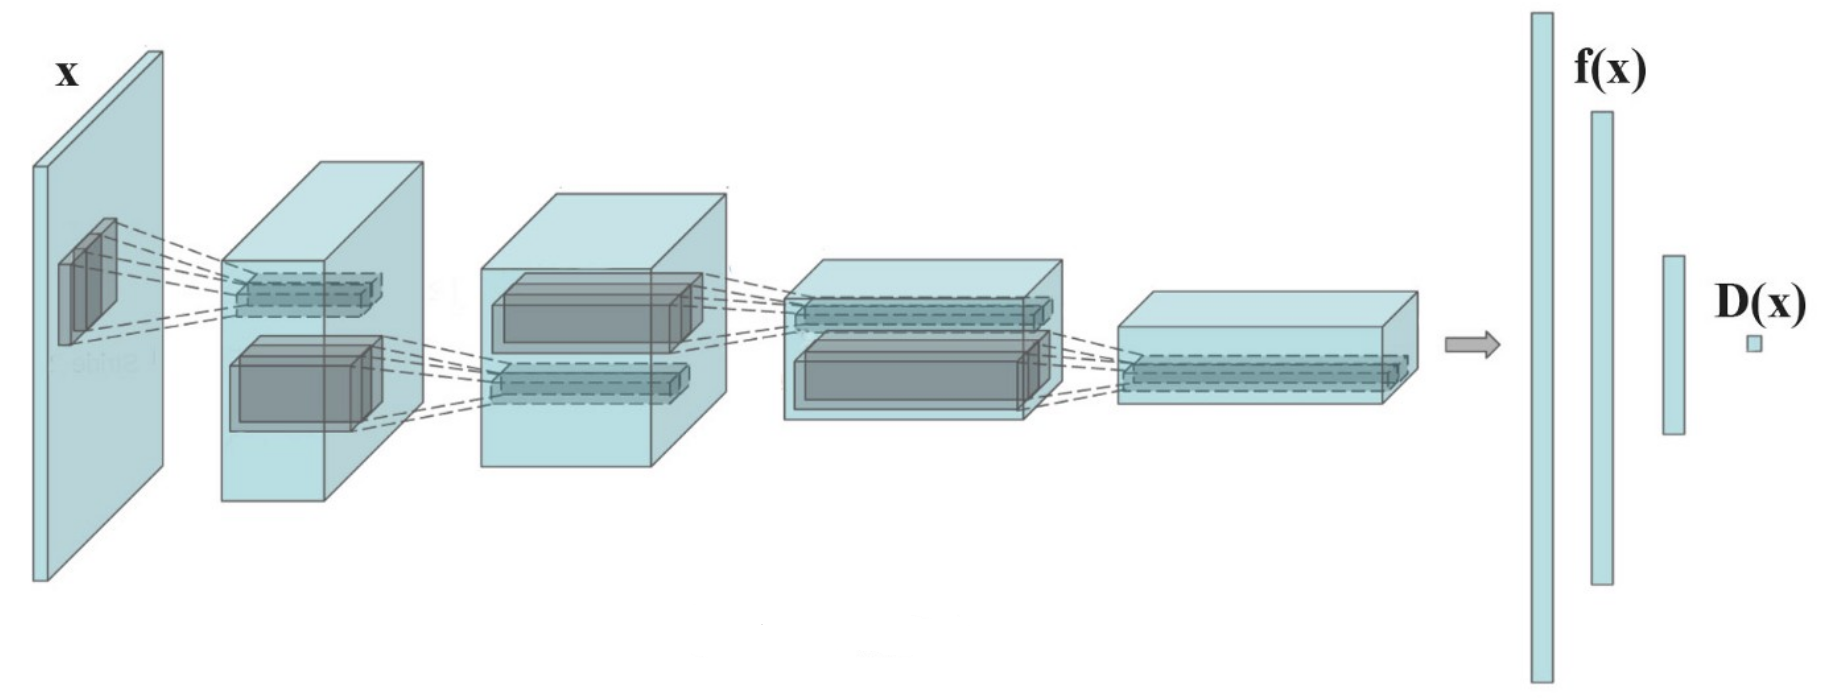
\includegraphics[scale = 0.4]{discriminador.png}
      \caption{Modelo Discriminador}
      \label{Alexis2}
    \end{center}
\end{figure}


Por el contrario, el generador es una red neuronal convolucional inversa, hace exactamente lo opuesto de lo que hace una CNN, ya que 
a estas se les da una imagen real como entrada y se espera una etiqueta clasificada como salida, 
pero en el generador, un vector de ruido aleatorio\emph{(z)} se da como señal de entrada 
y se espera una imagen falsa como salida, esta imagen deberá aproximarse a la real a
partir de una distribución $P(z)$ (en general una distribución Gaussiana) que
produce una muestra de datos falsos,$\tilde{x}$ es decir:

\begin{equation}
G(z) = \tilde{x}
\end{equation}

\begin{figure}[H]
    \begin{center}
      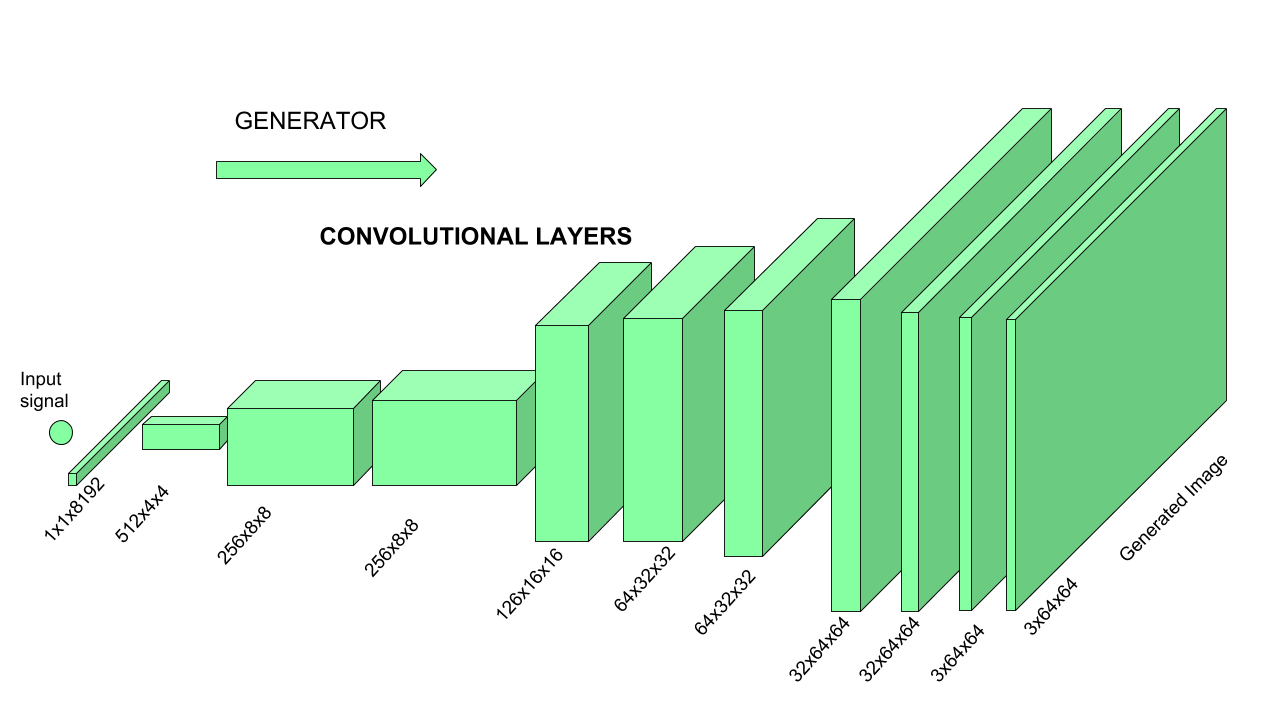
\includegraphics[scale = 0.6]{generador.png}
      \caption{Modelo Generador}
      \label{Alexis3}
    \end{center}
\end{figure}
    
\subsubsection{Funciones de perdida.}

Como parte del entrenamiento se necesitan parámetros que nos describan de manera correcta los resultados
que obtenemos de la predicción en nuestra red neuronal, para esto se hace el uso de funciones de perdida, estas funciones 
evalúan la desviación entre las predicciones realizadas por la red neuronal y los valores 
reales de las observaciones utilizadas durante el aprendizaje. A esta función se le conoce como perdida perceptual. Cuanto menor es el resultado de esta función, 
más eficiente es la red neuronal. Su minimización, es decir, reducir al mínimo la desviación entre el valor de la predicción y
el valor real para una observación dada, se hace ajustando los distintos pesos de la red neuronal.

En el caso de las redes adversarias, específicamente en \emph{SRGAN}, esta perdida es la suma de las perdidas de contenido $l_{X}^{SR}$ 
y las adversarias $10^{-3}l_{Gen}^{SR}$.


\begin{equation}
  l^{SR}=l_{X}^{SR} + 10^{-3}l_{Gen}^{SR}
\end{equation}


Como mencionan Goodfellow et al. \cite{GANs}, se tienen 
2 perdidas principales: La de contenido (\emph{content loss}), la cual se aproxima a una perdida perceptual mediante la perdida
de la red neuronal (\emph{VGG}),definimos entonces la perdida \emph{VGG} como la distancia euclidiana entre la representación de
características de una imagen reconstruida $G_{\theta G}(l^{LR})$ y la imagen de referencia o real $l^{HR}$.


\begin{equation}
  l_{VGG/i.j}^{SR}=\frac{1}{W_{i,j}H_{i,j}} \sum_{x=1}^{W_{i,j}}\sum_{y=1}^{H_{i,j}}(\phi_{i,j}(l^{HR})_{x,y}-\phi_{i,j} 
  (G_{\theta G}(l^{LR}))_{x,y})^{2}
\end{equation}

    
\subsubsection{Función de activación, Normalización y b}


